% generated by scripts/pkl_to_latex.py
% source PKL : tscan_v1_L6_Ne6_U1_mode-uniform_nmin2_solver-gcg_full_es_restarts8_iter300_kmax2_tol1em09_t0.1to15_N20-8b4145d60051.pkl
% scan type  : tscan
% state      : ex_singlet
% requires   : \usepackage{pgfplots} \pgfplotsset{compat=1.18}
% colours match the matplotlib PDF (tab10 cycle)
\definecolor{gmeC0}{HTML}{1F77B4}
\definecolor{gmeC1}{HTML}{FF7F0E}
\definecolor{gmeC2}{HTML}{2CA02C}
\definecolor{gmeC3}{HTML}{D62728}
\definecolor{gmeC4}{HTML}{9467BD}
\definecolor{gmeC5}{HTML}{8C564B}
\definecolor{gmeC6}{HTML}{E377C2}
\definecolor{gmeC7}{HTML}{17BECF}

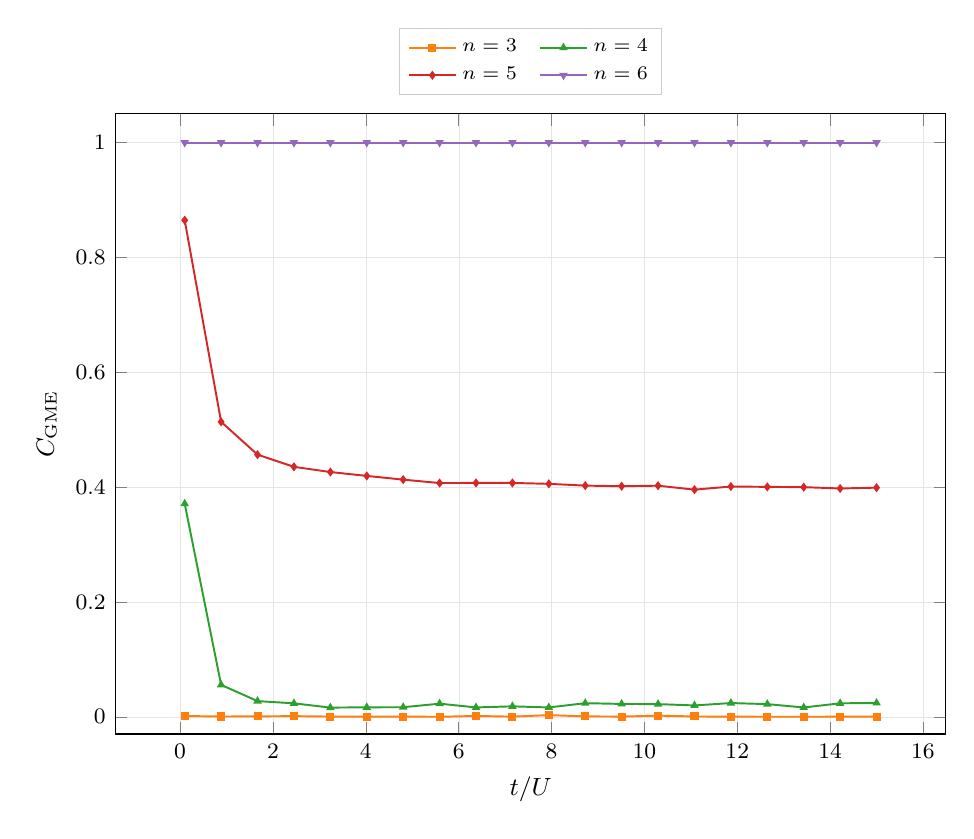
\begin{tikzpicture}
  \begin{axis}[
    width=\columnwidth,
    height=0.78\columnwidth,
    xlabel={$t/U$},
    ylabel={$C_{\mathrm{GME}}$},
    grid=both,
    grid style={line width=.1pt, draw=gray!20},
    tick label style={font=\footnotesize\rmfamily, /pgf/number format/fixed},
    label style={font=\small\rmfamily},
    scaled ticks=false,
    legend style={font=\scriptsize\rmfamily, draw=gray!40, at={(0.5,1.03)}, anchor=south, /tikz/every even column/.append style={column sep=6pt}},
    legend cell align={left},
    legend columns=2,
    ymin=-0.03,
    ymax=1.05,
  ]
    \addplot[color=gmeC1, mark=square*, mark size=1.1pt, line width=0.7pt] coordinates {
        (0.1,0.001392) (0.884211,0.000519) (1.668421,0.000782) (2.452632,0.001169)
        (3.236842,0.000424) (4.021053,0.000183) (4.805263,0.000376) (5.589474,0.000023)
        (6.373684,0.001489) (7.157895,0.000291) (7.942105,0.002937) (8.726316,0.000722)
        (9.510526,0.000392) (10.294737,0.002026) (11.078947,0.000596) (11.863158,0.000256)
        (12.647368,0.000113) (13.431579,0.000083) (14.215789,0.000208) (15,0.000289)
    };
    \addlegendentry{$n=3$}
    \addplot[color=gmeC2, mark=triangle*, mark size=1.1pt, line width=0.7pt] coordinates {
        (0.1,0.371043) (0.884211,0.055609) (1.668421,0.027349) (2.452632,0.023474)
        (3.236842,0.016035) (4.021053,0.016519) (4.805263,0.016701) (5.589474,0.022887)
        (6.373684,0.016342) (7.157895,0.01821) (7.942105,0.016305) (8.726316,0.023719)
        (9.510526,0.022426) (10.294737,0.022087) (11.078947,0.019797) (11.863158,0.023976)
        (12.647368,0.022082) (13.431579,0.016258) (14.215789,0.023512) (15,0.024088)
    };
    \addlegendentry{$n=4$}
    \addplot[color=gmeC3, mark=diamond*, mark size=1.1pt, line width=0.7pt] coordinates {
        (0.1,0.864713) (0.884211,0.51367) (1.668421,0.456538) (2.452632,0.435309)
        (3.236842,0.426263) (4.021053,0.419501) (4.805263,0.413029) (5.589474,0.40707)
        (6.373684,0.407309) (7.157895,0.407254) (7.942105,0.405704) (8.726316,0.402581)
        (9.510526,0.401526) (10.294737,0.40247) (11.078947,0.395562) (11.863158,0.401028)
        (12.647368,0.40044) (13.431579,0.399922) (14.215789,0.397641) (15,0.399048)
    };
    \addlegendentry{$n=5$}
    \addplot[color=gmeC4, mark=triangle*, mark size=1.1pt, mark options={rotate=180}, line width=0.7pt] coordinates {
        (0.1,1) (0.884211,1) (1.668421,1) (2.452632,1)
        (3.236842,1) (4.021053,1) (4.805263,1) (5.589474,1)
        (6.373684,1) (7.157895,1) (7.942105,1) (8.726316,1)
        (9.510526,1) (10.294737,1) (11.078947,1) (11.863158,1)
        (12.647368,1) (13.431579,1) (14.215789,1) (15,1)
    };
    \addlegendentry{$n=6$}
  \end{axis}
\end{tikzpicture}
